\documentclass{beamer}
\usetheme{Madrid}

\usepackage{amsmath, amssymb, amsthm}
\usepackage{graphicx}
\usepackage{listings}
\usepackage{gensymb}
\usepackage[utf8]{inputenc}
\usepackage{hyperref}
\usepackage{gvv}
\usepackage{tikz}
\lstset{
  language=Python,
  basicstyle=\ttfamily\small,
  keywordstyle=\color{blue},
  stringstyle=\color{orange},
  numbers=left,
  numberstyle=\tiny\color{gray},
  breaklines=true,
  showstringspaces=false
}
\usetikzlibrary{decorations.pathmorphing}

\title{Question-1.5.10}
\author{EE25BTECH11022 - sankeerthan}
\date{}
\begin{document}

\frame{\titlepage}

\begin{frame}
\frametitle{Question}
Find the ratio in which the line segment joining the points $\vec{A}$\brak{1, -5} and $\vec{B}$\brak{-4, 5} is divided by X-axis. Also,find the coordinates of the  point of division.
\end{frame}

\begin{frame}
\frametitle{Solution}
Let the given points be A and B
\begin{align*} \vec{A} = \myvec{1 \\ -5}, \vec{B} = \myvec{-4 \\ 5} \end{align*}
Let the X-axis divide the line segment \(\overline{\vec{AB}}\) at point $\vec{P}$ in the ratio $k:1$.
Since $\vec{P}$ lies on X-axis, let
\begin{align*}
\vec{P} = \myvec{x \\ 0}
\end{align*}
The point $\vec{A}$, $\vec{B}$, $\vec{P}$ are collinear.
\begin{align}
\implies \text{rank}\myvec{\vec{B}-\vec{A} & \vec{P}-\vec{A}} = 1
\end{align}
\end{frame}

\begin{frame}
\frametitle{Solution}
\begin{align}
\myvec{-5 & x-1 \\ 10 & 5} \xleftrightarrow{R_1 \rightarrow {R_1 + \frac{1}{2}R_2}}\myvec{0 & x-\frac{3}{2} \\ 10 & 5} \xleftrightarrow{R_1 \leftrightarrow R_2}  \myvec{10 & 5 \\ 0 & x-\frac{3}{2}} 
\end{align}
The number of nonzero rows in the row reduced matrix (also known as {\em echelon form}) is defined as the rank. For above matrix to be of rank 1,
\begin{align}
x+\frac{3}{2} &= 0 \\
x &= \frac{-3}{2}
\end{align}
$\therefore$ The coordinates of the point of intersection are 
\begin{align*}
\vec{P} = \myvec{\frac{-3}{2} \\ 0}
\end{align*}
\end{frame}

\begin{frame}
\frametitle{Solution}
Substituting the values of $\vec{A}$, $\vec{B}$ and $\vec{P}$,
\begin{align}
k=\frac{\myvec{\frac{5}{2} & -5}\myvec{\frac{5}{2} \\ -5}}{\norm{\myvec{\frac{5}{2} \\ -5}}^2}=1
\end{align}

Thus, the ratio in which the point $\vec{P}$ divides the line segment $\vec{AB}$ is \textbf{1:1}. 
\end{frame}

\begin{frame}
\frametitle{graph}
\begin{figure}[!ht]
    \centering
    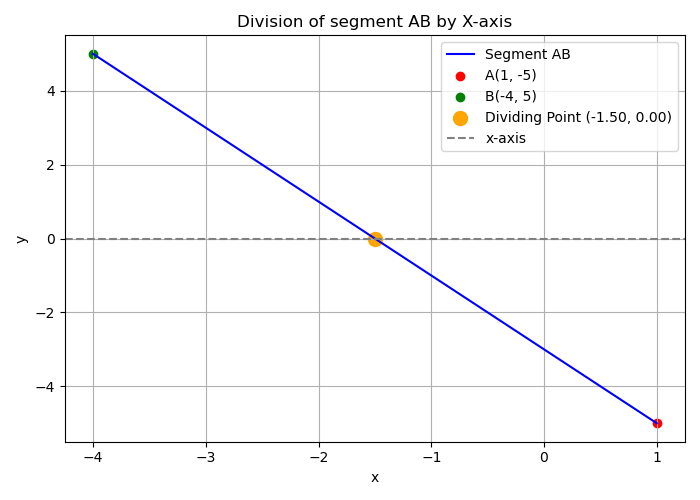
\includegraphics[width=\linewidth]{figs/points.png}
    \caption{Ellipse bounded region}
\end{figure}
\end{frame}

\begin{frame}[fragile]
\frametitle{C-Code}
\begin{lstlisting}[language=C]
#include <stdio.h>

void division_point(double *A, double *B, double *P, double *k) {
    *k = -A[1] / B[1];
    P[0] = ((*k) * B[0] + A[0]) / ((*k) + 1);
    P[1] = 0;
}

int main() {
    double A[2] = {1, -5};
    double B[2] = {-4, 5};
        double P[2];
    double k;
     division_point(A, B, P, &k);
    printf("Ratio: %f : 1\n", k);
    printf("Division Point: (%f, %f)\n", P[0], P[1]);
    return 0;
}
 \end{lstlisting}
\end{frame}

\begin{frame}[fragile]
\frametitle{Python-Code}
\begin{lstlisting}
# Code by GVV Sharma
# Modified for Problem Solution
# Released under GNU GPL
# Calculating area enclosed between curves
import ctypes
import numpy as np

lib = ctypes.cdll.LoadLibrary('./code.so')

lib.division_point.argtypes = [
    ctypes.POINTER(ctypes.c_double),
    ctypes.POINTER(ctypes.c_double),
    ctypes.POINTER(ctypes.c_double),
    ctypes.POINTER(ctypes.c_double)]
lib.division_point.restype = None

\end{lstlisting}
\end{frame}

\begin{frame}[fragile]
\frametitle{Python-Code}
\begin{lstlisting}
def get_points():
    A = np.array([1, -5], dtype=np.double)
    B = np.array([-4, 5], dtype=np.double)
    P = np.zeros(2, dtype=np.double)
    k = ctypes.c_double()
    lib.division_point(A.ctypes.data_as(ctypes.POINTER(ctypes.c_double)),
                       B.ctypes.data_as(ctypes.POINTER(ctypes.c_double)),
                       P.ctypes.data_as(ctypes.POINTER(ctypes.c_double)),
                       ctypes.byref(k))
    return P, k.value, A, B
\end{lstlisting}
\end{frame}

\begin{frame}[fragile]
\frametitle{Python-Code}
\begin{lstlisting}
import matplotlib.pyplot as plt
import numpy as np
from call import get_points

P, k, A, B = get_points()

plt.figure(figsize=(7,5))
plt.plot([A[0], B[0]], [A[1], B[1]], 'b-', label='Segment AB')
plt.scatter(A[0], A[1], color='red', label='A(1, -5)')
plt.scatter(B[0], B[1], color='green', label='B(-4, 5)')
plt.scatter(P[0], P[1], color='orange', s=100, label=f'Dividing Point ({P[0]:.2f}, {P[1]:.2f})')

\end{lstlisting}
\end{frame}

\begin{frame}[fragile]
\frametitle{Python-Code}
\begin{lstlisting}
plt.axhline(0, color='gray', ls='--', label='x-axis')
plt.xlabel('x')
plt.ylabel('y')
plt.title('Division of segment AB by X-axis')
plt.legend()
plt.grid(True)
plt.tight_layout()
plt.show()

\end{lstlisting}
\end{frame}

\end{document}